\section{SWID Erweiterung}
\label{swiderweiterung}

\section{Datenmodell}
Die Erweiterung des bestehenden Datenmodells ist in \autoref{fig:database-model}
zu sehen. Die hinzugefügten Tabellen sind durch den grünen Hintergrund
hervorgehoben. Bei Tabellen mit grauem Rahmen handelt es sich um
Zwischentabellen, welche eine N zu M Beziehung auflösen.\\
Beim Modellieren der zusätzlichen Tabellen wurde darauf geachtet, dass keine der
bestehenden Tabellen angepasst werden mussten. Die Beziehungen werden daher alle
von der Seite der Erweiterung hergestellt.

\begin{figure}[H]
	\centering
	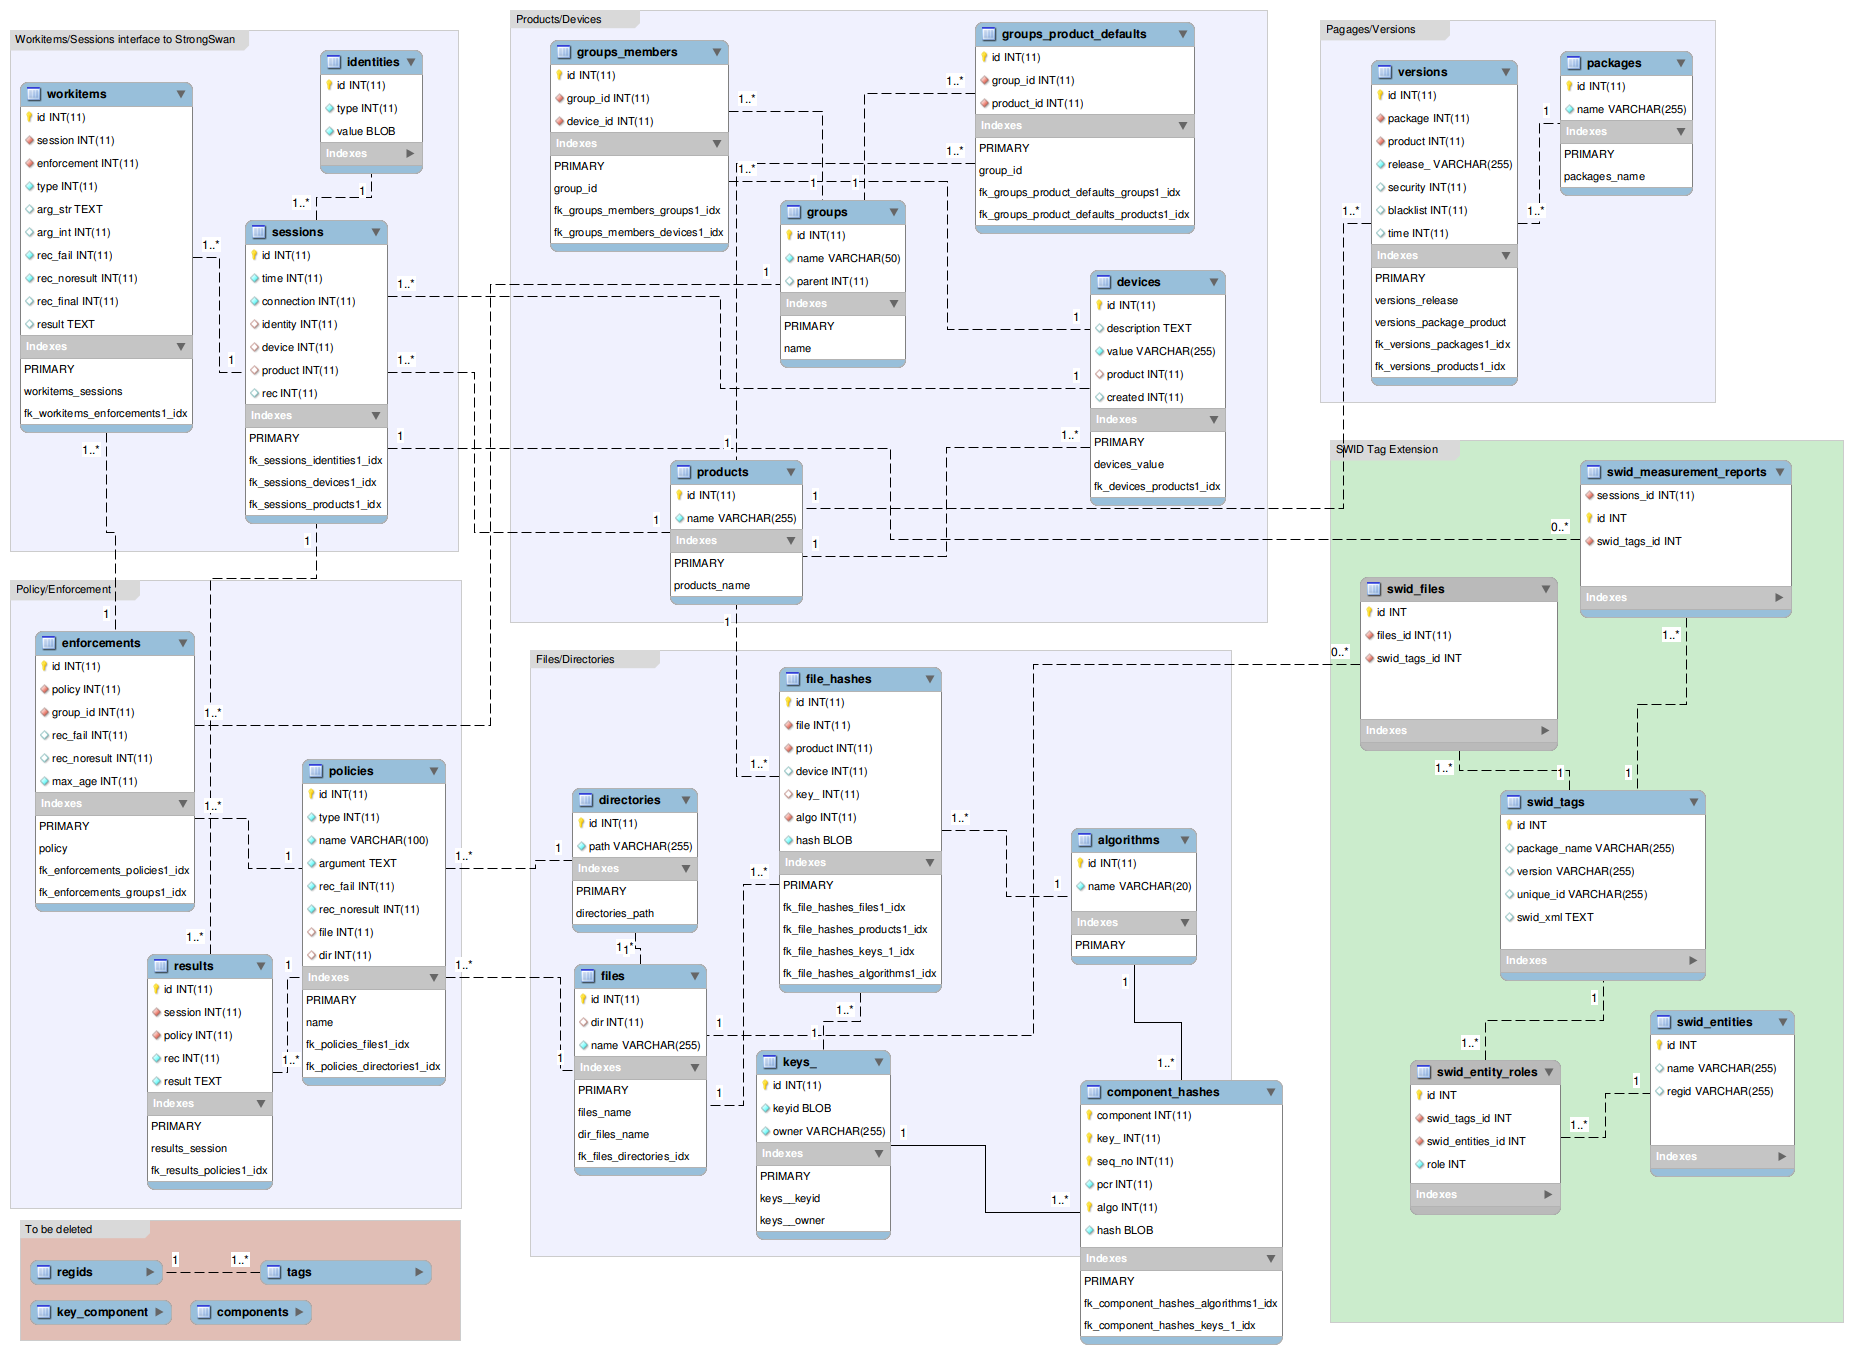
\includegraphics[angle=90,width=0.8\textwidth]{./images/db/database-model}
	\caption{Bestehendes Datenmodel inklusive SWID Erweiterung (grün)}
	\label{fig:database-model}
\end{figure}

\begin{description}
	
	\item[swid\_entity] Diese Tabelle beinhaltet alle erfassten Entities. In der
	Regel ist eine kleine Anzahl unterschiedlicher Entities zu erwarten, weshalb
	diese in einer eigenen Tabelle gehalten werden und über die swid\_entityroles
	mit den SWID Tags verknüpft werden.

	\item [swid\_entityroles] Ein SWID Tag kann mehrere Entities enthalten.
	Entities nehmen in einem Tag eine oder eine Kombination von Rollen ein. Es
	existieren die Rollen Tag Creator, Licensor und Publisher. Pro SWID Tag darf es
	nur einen Tag Creator geben. Diese Einschränkung wird jedoch erst in den Django
	Models durch das ORM angewendet.

	\item [swid\_tags\_files] In dieser Tabelle wird die Beziehung zwischen einem
	File und einem SWID Tag erfasst. Ein SWID Tag kann mehrere Files beinhalten
	(\nameref{strongTNC:UC04}).

	\item[swid\_tags\_sessions] Bei der Durchführen einer Messung von SWID Tags
	werden die entsprechenden Tags in dieser Tabelle abgespeichert
	(\nameref{strongTNC:UC06}). Hier werden die gemessenen Tags mit passenden
	Session verknüpft.

\end{description}


\section{Architektur SWID Messung}

\begin{figure}[H]
	\centering
	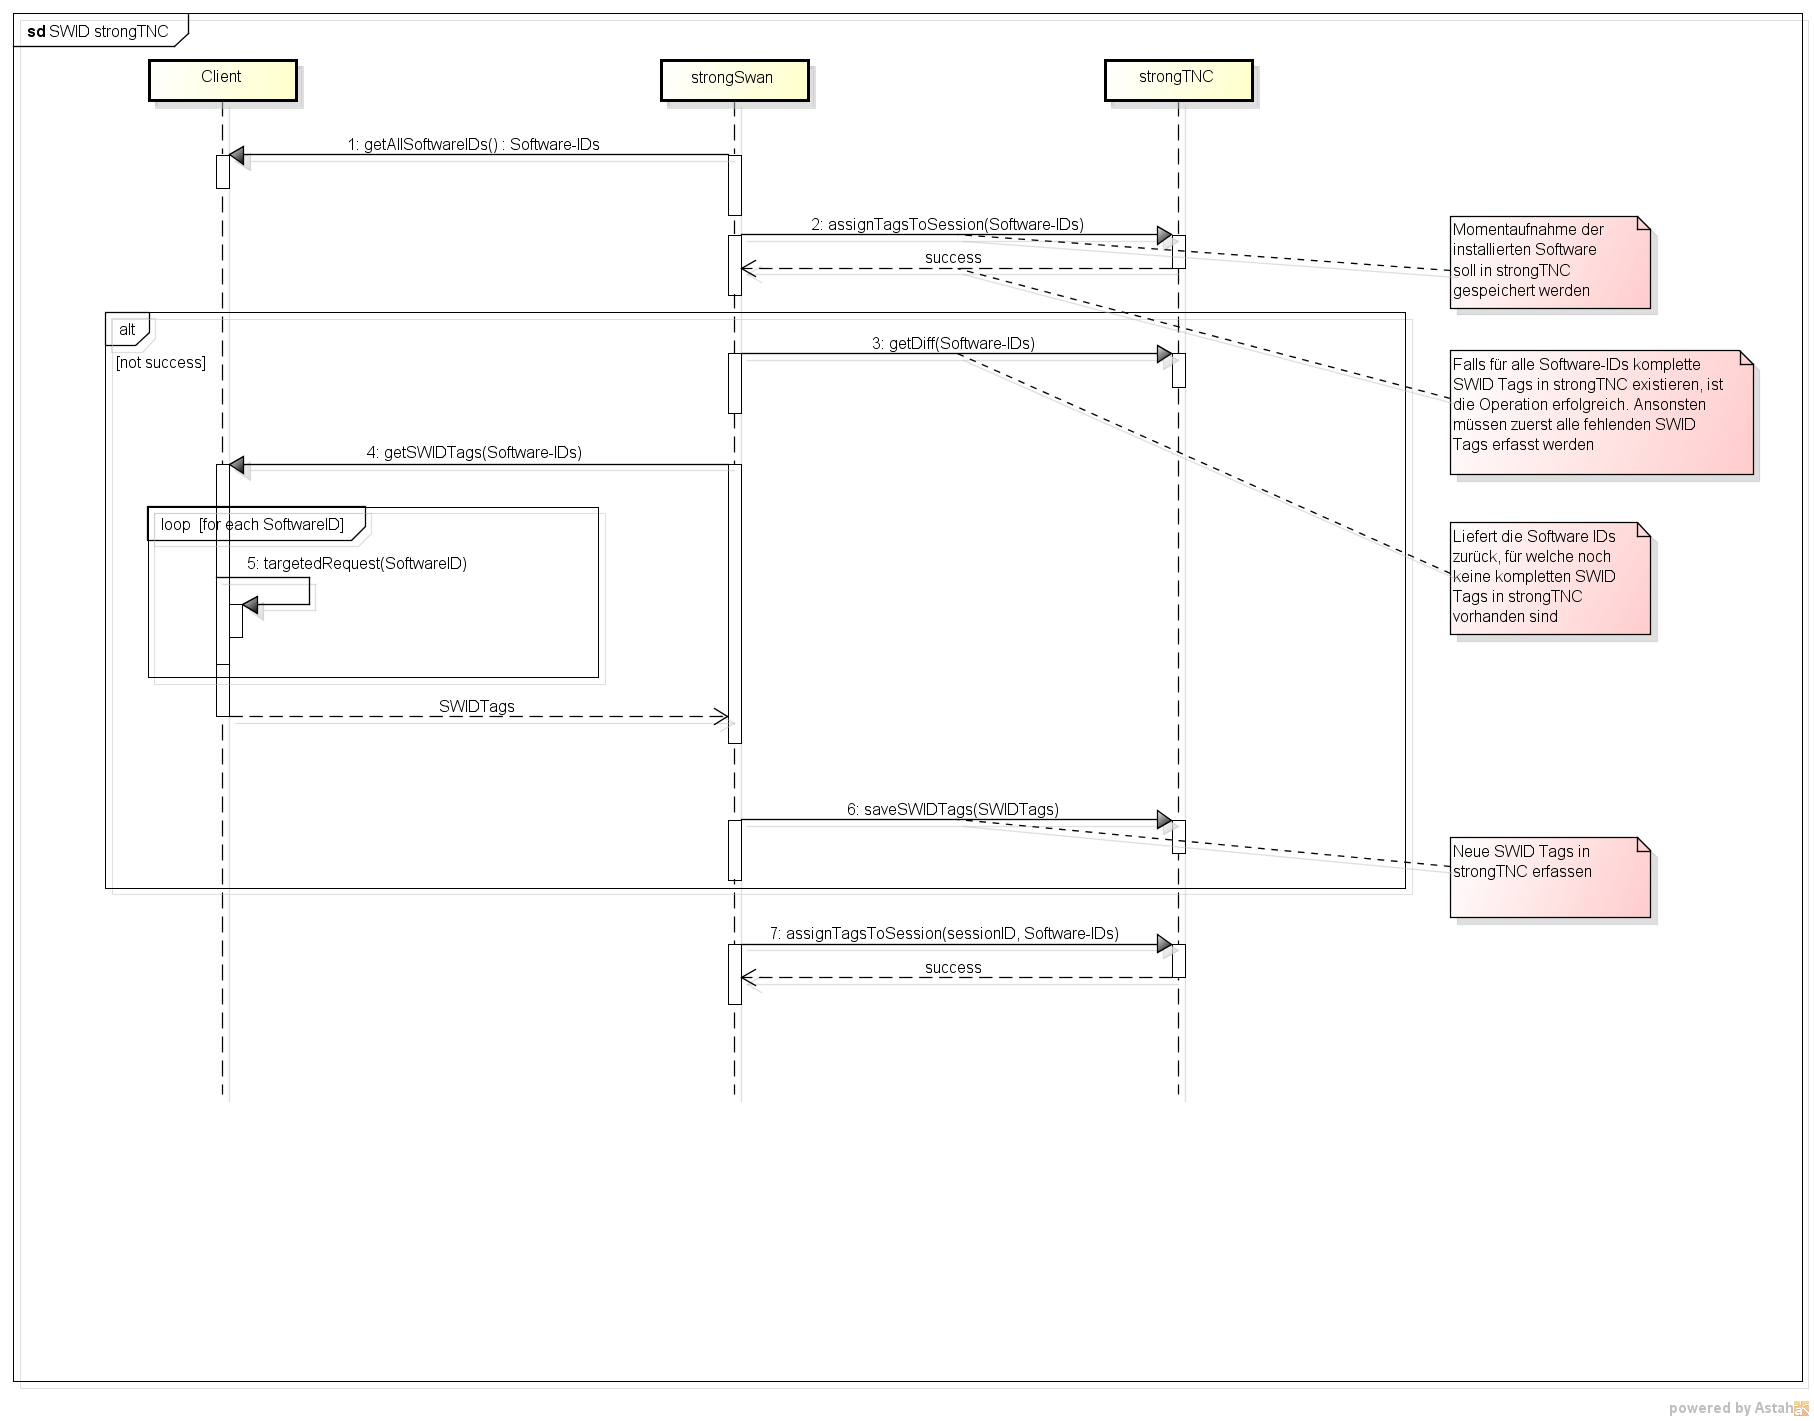
\includegraphics[width=0.9\textwidth]{./images/architecture/SWID_strongTNC.png}
	\caption{Ablauf einer SWID Tag Messung}
	\label{fig:swid-measurement}
\end{figure}

In \autoref{fig:swid-measurement} ist der Ablauf der SWID Tag Messung
(\nameref{strongTNC:UC06}) ersichtlich. Eine Messung läuft wie folgt ab:

\begin{enumerate}
	\item Auf dem Client werden die Software-IDs aller installierten Pakete generiert. 
	
	\item Es wird versucht die Liste der generierten Software-IDs mit einer Session
	zu verknüpfen.
	\begin{description*}
		\item[2a] Existiert zu allen Software-IDs ein entsprechender SWID Tag, ist die
		Messung abgeschlossen und die SWID Tags sind mit der Session verknüpft. Es
		sind keine weiteren Schritte mehr nötig (ENDE).
		
		\item[2b] Existiert für mindestens eine Software-ID kein entsprechender SWID
		Tag, wird die Messung abgebrochen und eine Liste jener Software-IDs, für
		welche kein SWID Tag existiert, zurückgeliefert. Weiter zu Punkt 3.
	\end{description*}
		
	\item Bevor die Messung durchgeführt werden kann, müssen alle fehlenden SWID
	Tags erfasst werden. Die einzelnen XML Dokumente der SWID Tags werden vom
	Client anhand sogenannter \enquote{Targeted Requests} (siehe Abschnitt
	\ref{swidgenerator:UC04}) erstellt, das heisst, der Generator kreiert gezielt
	die Tags für die gegebenen Software-IDs und nicht für alle installierten
	Software Pakete.
	
	\item Der Client erfasst alle neu generierten SWID Tags in strongTNC.
	
	\item Der Client startet erneut eine Messung und übermittelt alle Software-IDs.
	Nun sind für alle Software-IDs die entsprechenden SWID Tags vorhanden und die
	Messung wird erfolgreich abgeschlossen. Ansonsten zurück zu Schritt 2.
\end{enumerate}

Dieses Vorgehen erzwingt eine Aktualisierung der strongTNC Datenbank falls diese
nicht alle SWID Tags enthält, bevor eine Messung erfolgreich abgeschlossen
werden kann. Dadurch wird erreicht, dass auf Serverseite kein Zustand gewahrt
werden muss, wie es für eine nicht abgeschlossene Messung, welche später
abgeschlossen wird, der Fall wäre. Dieses Vorgehen entspricht den Prinzipien von
HTTP, eine Messung kann jederzeit durchgeführt werden, ohne dass ein Zustand
oder Kontextinformationen vorhanden sein müssen. Das heisst, wenn eine Messung
nicht vollständig und korrekt durchgeführt werden kann, werden keine Daten
verändert.

\subsection{Technische Umsetzung}
Der Zugriff auf die beschriebene Systemoperation erfolgt durch die, in dieser
Arbeit ausgearbeiteten, RESTful HTTP Schnittstelle. Das komplette Konzept ist in
Anhang (\autoref{REST:api-konzept}) zu finden.

\subsubsection{REST Kommunikation}
Im Folgenden soll der Ablauf einer Messung anhand eines konkreten Beispiels
illustriert werden. In diesem Beispiel erfolgt eine Messung für drei Tags mit
folgenden Software-IDs:

\begin{textcode}
regid.2004-03.org.strongswan Ubuntu 12.04-i686-logrotate-3.7.8-6ubuntu5
regid.2004-03.org.strongswan Ubuntu 12.04-i686-lsb-base-4.0-0ubuntu20
regid.2004-03.org.strongswan Ubuntu 12.04-i686-strongswan-4.5.2-1.5+deb7u3
\end{textcode}

Der HTTP Endpunkt wurde wie folgt definiert:

\begin{mdframed}[style=def]
\begin{description*}
	\item[URI Path] \texttt{/sessions/\{id\}/register-swid-measurement/}
	\item[Archetype] Controller
	\item[Methods] POST
	\item[Content-Type] \texttt{application/json; charset=utf-8}
	\item[Request Parameter] \hfill
	\begin{description*}
		\item[\texttt{softwareId}] Software-IDs als JSON-Liste.
	\end{description*}
	\item[Response Statuscodes] \hfill
		\begin{description*}
			\item[200 OK] SWID Tags der übermittelten Software-IDs sind eingetragen \\
				und wurden für die übermittelte Session eingetragen
			\item[404 Not Found] Session mit der spezifizierten ID wurde nicht gefunden. 
			\item[412 Precondition Failed] Es existieren nicht alle SWID Tags für die
				übertragenen Software-IDs. Als Payload werden die fehlenden Software-IDs
				übertragen.
		\end{description*}
	\item[JSON Format Response] \hfill
	
\begin{jsoncode}
{"data" : 
	[
		"regid.2004-03.org.strongswan Ubuntu 12.04-i686-logrotate-3.7.8-6ubuntu5",
		"regid.2004-03.org.strongswan Ubuntu 12.04-i686-lsb-base-4.0-0ubuntu20",
		"regid.2004-03.org.strongswan Ubuntu 12.04-i686-strongswan-4.5.2-1.5+deb7u3" 
	]
}
\end{jsoncode}
\end{description*}
\end{mdframed}

\paragraph{Übermitteln von Software-IDs} \hspace{0pt} \\
Die Daten werden als JSON-Liste an den entsprechenden Endpunkt gesendet.
Der HTTP Request sieht folgendermassen aus:

\begin{listing}
\caption{Übermitteln von Software-IDs via REST API}
\begin{httpcode}
POST /api/sessions/2/swid-measurement/ HTTP/1.1
Authorization: Basic cm9vdDpyb290
Host: tncserver:8000
Accept: application/json
Content-Type: application/json; charset=utf-8
Content-Length: 232

{
	"data":
	[
		"regid.2004-03.org.strongswan_Ubuntu_12.04-i686-logrotate-3.7.8-6ubuntu5",
		"regid.2004-03.org.strongswan_Ubuntu_12.04-i686-lsb-base-4.0-0ubuntu20",
		"regid.2004-03.org.strongswan_Ubuntu_12.04-i686-strongswan-4.5.2-1.5+deb7u3"
	]
}
\end{httpcode}
\end{listing}

Der entsprechende cURL\footnote{\url{http://curl.haxx.se/}} Befehl:

\begin{bashcode}
curl -i -X POST https://strongtnc/api/sessions/2/swid-measurement/ \
		 -u username:password \
		 -H "Accept: application/json" \
		 -H "Content-Type: application/json; charset=utf-8" \
		 -d "$DATA"
\end{bashcode}


\paragraph{Antwort - Status 412 Precondition Failed} \hspace{0pt} \\
Sind noch nicht alle Tags in der strongTNC Datenbank vorhanden, werden die
Software-IDs der fehlenden Tags zurückgeliefert. Der HTTP Status Code ist
\texttt{412 Precondition Failed}. Es werden zu diesem Zeitpunkt noch keine Tags
mit der Session verknüpft. Eine entsprechende Antwort kann wie folgt aussehen:

\begin{listing}
\caption{HTTP Response mit Status Code 412 PRECONDITION FAILED}
\begin{httpcode}
HTTP/1.0 412 PRECONDITION FAILED
Date: Wed, 14 May 2014 15:21:45 GMT
Server: WSGIServer/0.1 Python/2.7
Vary: Accept, Cookie
Content-Type: application/json
Allow: POST, OPTIONS

["regid.2004-03.org.strongswan_Ubuntu_12.04-i686-strongswan-4.5.2-1.5+deb7u3"]
\end{httpcode}
\end{listing}

\paragraph{Antwort - Status 200 OK} \hspace{0pt} \\

Sind für alle Software-IDs bereits Tags in der Datenbank vorhanden, würde die
Antwort wie folgt aussehen:

\begin{listing}
\caption{HTTP Response mit Status Code 200 OK}
\begin{httpcode}
HTTP/1.0 200 OK
Date: Wed, 14 May 2014 15:21:45 GMT
Server: WSGIServer/0.1 Python/2.7
Vary: Accept, Cookie
Content-Type: application/json
Allow: POST, OPTIONS

[]
\end{httpcode}
\end{listing}

\paragraph{Nacherfassen von SWID Tags}\hspace{0pt} \\
War die Messung nicht erfolgreich (\texttt{HTTP 412}), müssen für die
zurückgelieferten Software-IDs zuerst komplette SWID Tags erfasst werden. Die
Daten für diesen Request bestehen aus einer JSON-Liste von XML Strings, dadurch
können auch mehrere Tags auf einmal erfasst werden. Empfehlenswert ist
allerdings eine Aufteilung in mehrere Gruppen, da die Requests sonst lange
dauern können.

Der Request sieht folgendermassen aus:

\begin{listing}
\caption{SWID Tags erfassen via REST API}
\begin{httpcode}
POST /api/swid/add-tags/ HTTP/1.1
Authorization: Basic cm9vdDpyb290
Host: tncserver:8000
Accept: application/json
Content-Type: application/json; charset="utf-8"
Content-Length: 239

{ "data" : 
	[
		"<?xml version=\"1.0\" encoding=\"utf-8\"?><SoftwareIdentity name=\"fortune-mod\"...",
		"<?xml version=\"1.0\" encoding=\"UTF-8\"?><SoftwareIdentity name=\"strongswan\"..."
	]
}

\end{httpcode}
\end{listing}

cURL Befehl:

\begin{bashcode}
curl -i -X POST https://strongtnc/api/swid/add-tags/ \
		 -u username:password \
		 -H "Accept: application/json" \
		 -H "Content-Type: application/json; charset=utf-8" \
		 -d "{ \"data\" : $DATA }"
\end{bashcode}

Eine ausführliche Spezifikation zur Kommunikation mit diesem REST Endpunkt ist
im Anhang \autoref{REST:swid-measurement-manual} zu finden. Darin sind unter
Anderem noch Informationen zu Fehlersituationen aufgeführt.


\subsection{SWID Views}
Für die SWID Tag Erweiterungen wurden drei neue Views implementiert. Mit diesen
Views können sämtliche ermittelten Usecases (Abschnitt~\ref{strongTCN:usecases})
abgedeckt werden.\\
Die Views sind visuell dem Stil der bereits vorhanden Templates angepasst.
Allerdings wurde für die Implementation der Views nicht der funktionsbasierte,
sondern der klassenbasierte Ansatz gewählt, wie in der Analyse erwähnt
(Abschnitt \ref{analyse:einschaezung}). Diese Views dienen somit also auch als
Vorlage, beziehungsweise Machbarkeitsnachweis für die Umsetzung mit
\enquote{Class Based Views}.


\subsubsection{Regid View}
Der Zweck der Regid Ansicht ist das Auflisten der im System vorhandenen Entities
mit Detailinformationen (\nameref{strongTNC:UC03}). Beim Wählen einer Entity
werden die referenzierten Tags aufgelistet, diese sind mit der Tag View
verknüpft.

\begin{figure}[H]
	\centering
	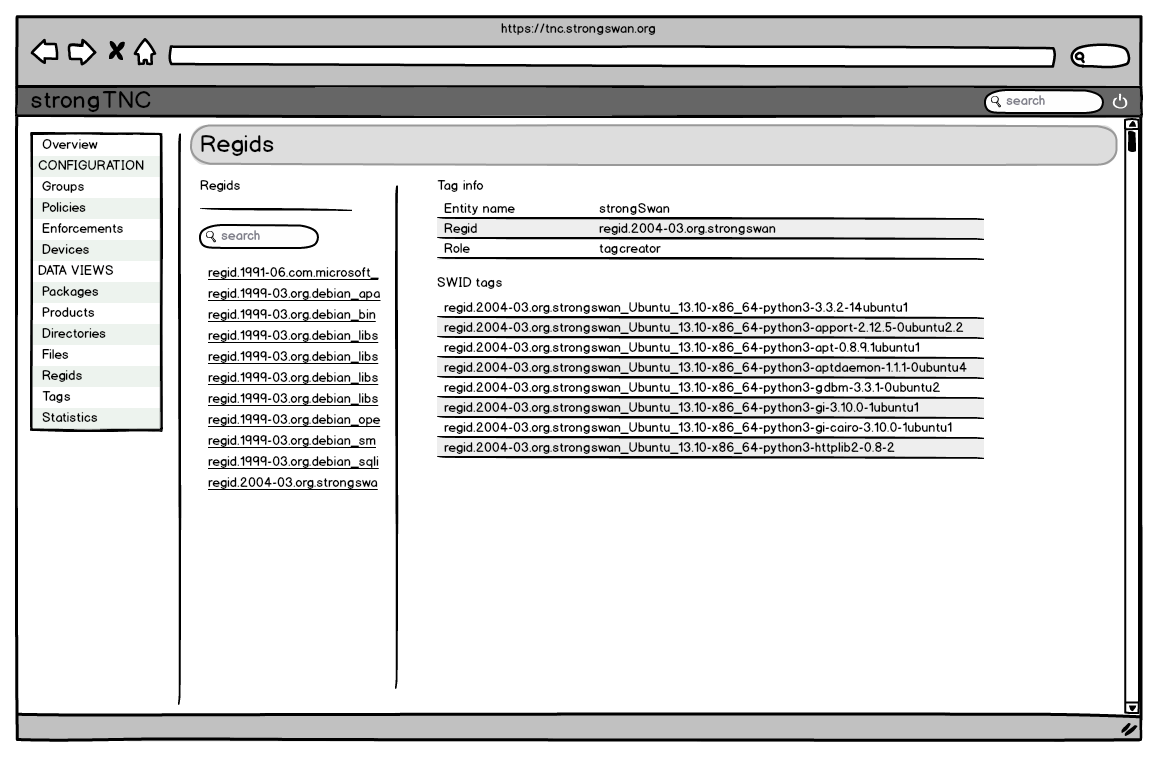
\includegraphics[width=0.8\textwidth]{./images/mockups/swid-regid-view}
	\caption{Mockup Regid View}
	\label{fig:regid-view-mockup}
\end{figure}

\begin{figure}[H]
	\centering
	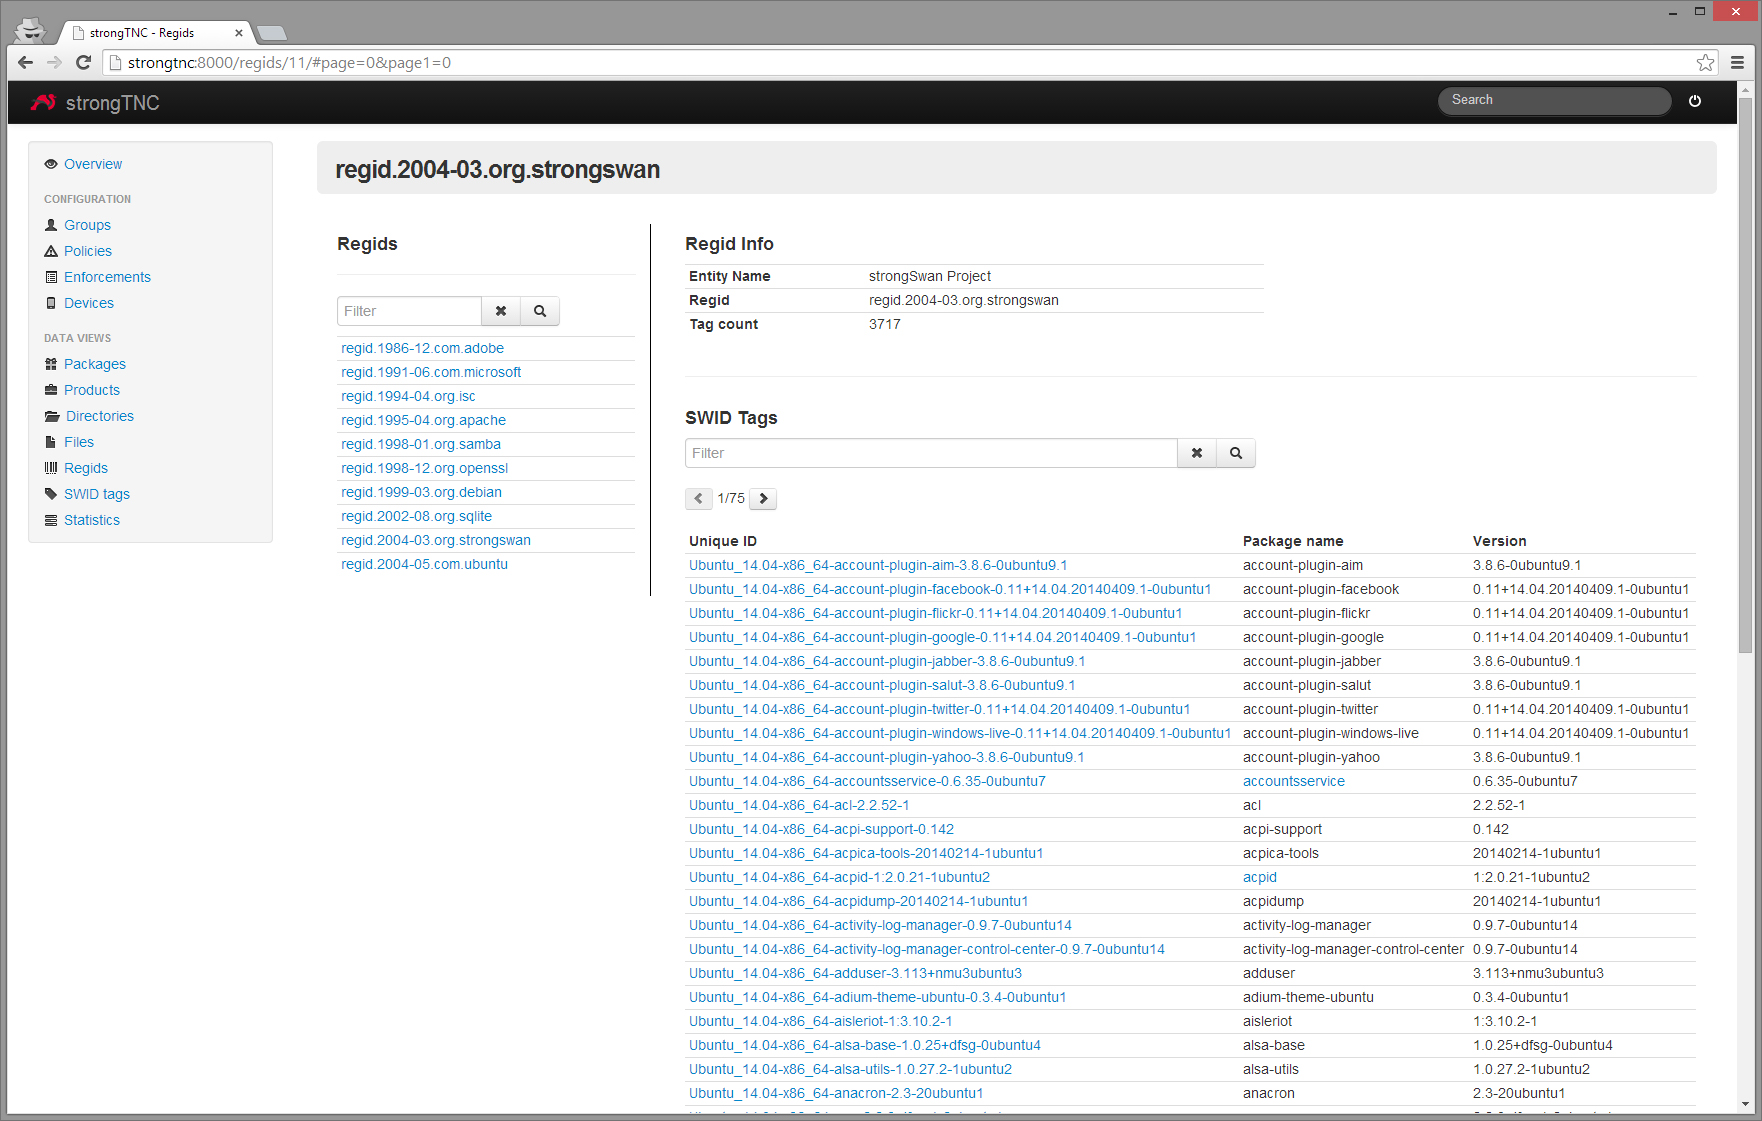
\includegraphics[width=0.8\textwidth]{./images/Views/regid-view}
	\caption{Regid View mit Detailansicht}
	\label{fig:regid-view}
\end{figure}


\subsubsection{SWID Tag View}
Der Zweck der SWID Tag Ansicht ist das Auflisten im System vorhandener SWID Tags
(\nameref{strongTNC:UC04}). Beim Auswählen eines SWID Tags werden
Detailinformationen angezeigt. So ist es möglich herauszufinden auf welchen
Geräten ein Tag registriert ist und welche Dateien zum jeweiligen Tag gehören.

\begin{figure}[H]
	\centering
	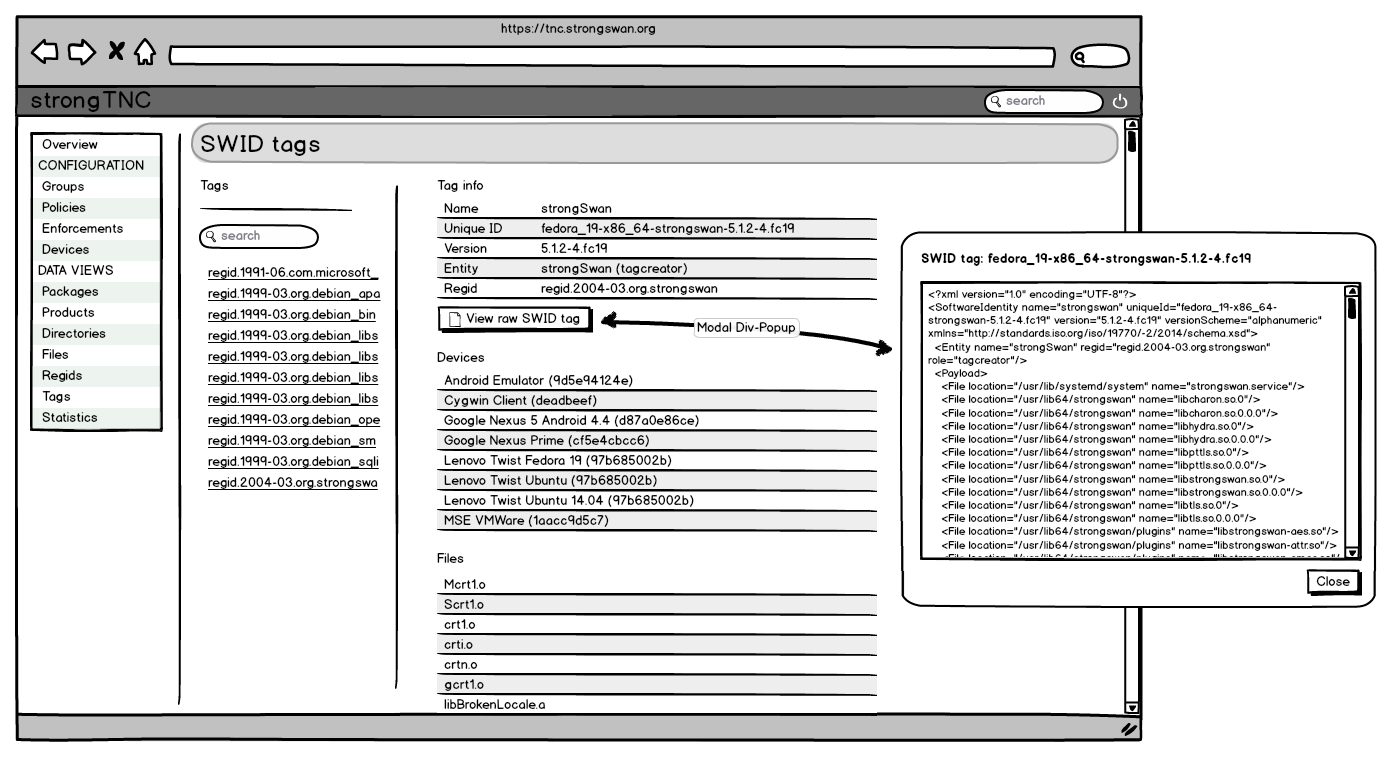
\includegraphics[width=0.9\textwidth]{./images/mockups/swid-tag-view}
	\caption{Mockup SWID Tag View}
	\label{fig:swid-tag-view-mockup}
\end{figure}

\begin{figure}[H]
	\centering
	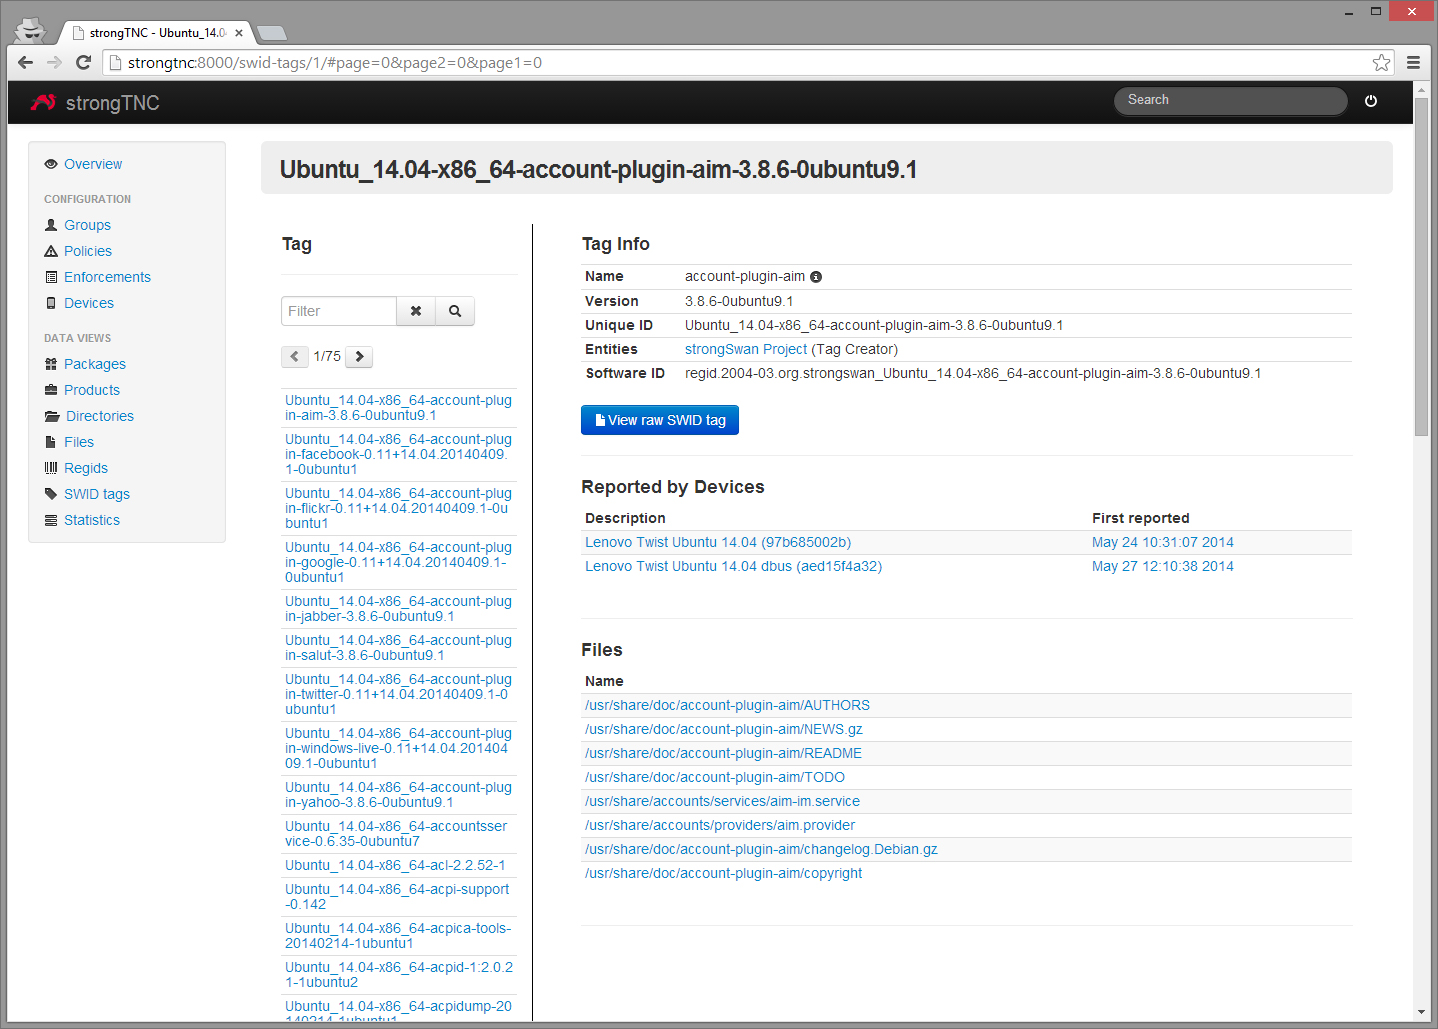
\includegraphics[width=0.8\textwidth]{./images/Views/tag-detail-view}
	\caption{SWID Tag View mit Details}
	\label{fig:swid-tag-view}
\end{figure}


\subsubsection{SWID Inventory View}
Mit Hilfe der SWID Inventory View kann festgestellt werden, welche Software für
eine ausgewählte Session auf einem Gerät installiert war
(\nameref{strongTNC:UC01}).\\
Mittels Datumsauswahl kann eingeschränkt werden welcher Bereich von Sessions
geladen werden soll. Die Tags der geladenen Sessions werden dynamisch
nachgeladen.

\begin{figure}[H]
	\centering
	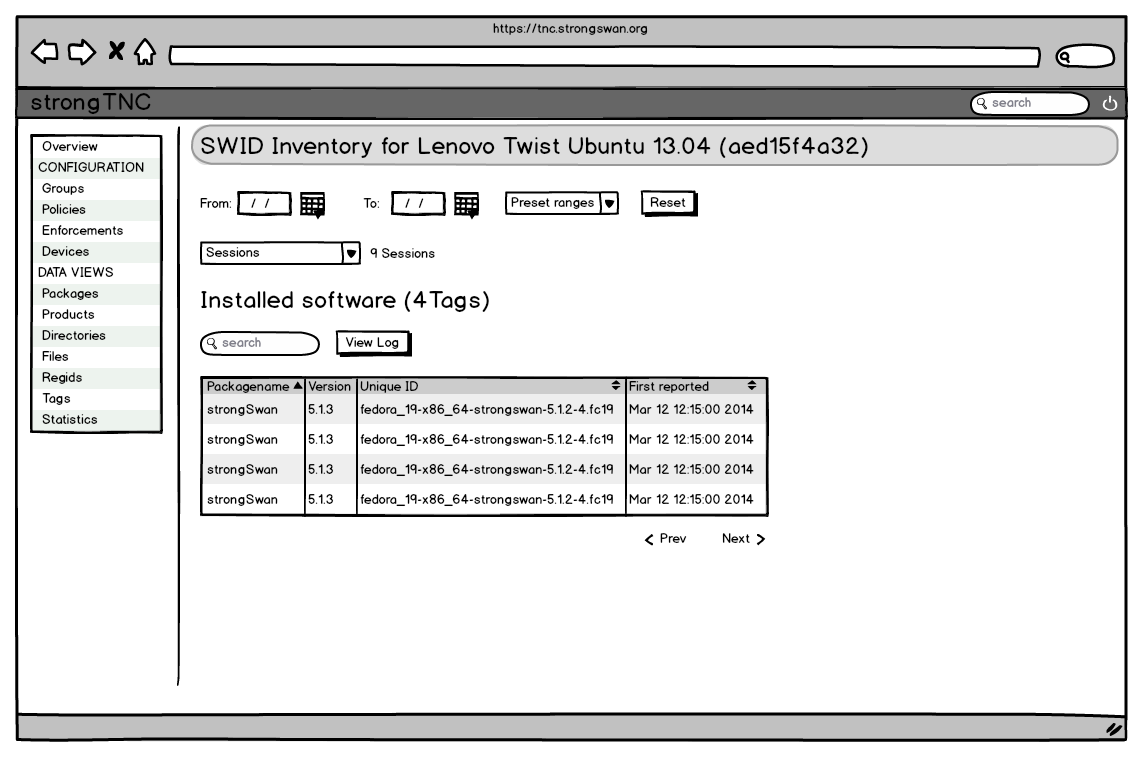
\includegraphics[width=0.8\textwidth]{./images/mockups/swid-inventory}
	\caption{Mockup SWID Inventory}
	\label{fig:swid-inventory-view-mockup}
\end{figure}

\begin{figure}[H]
	\centering
	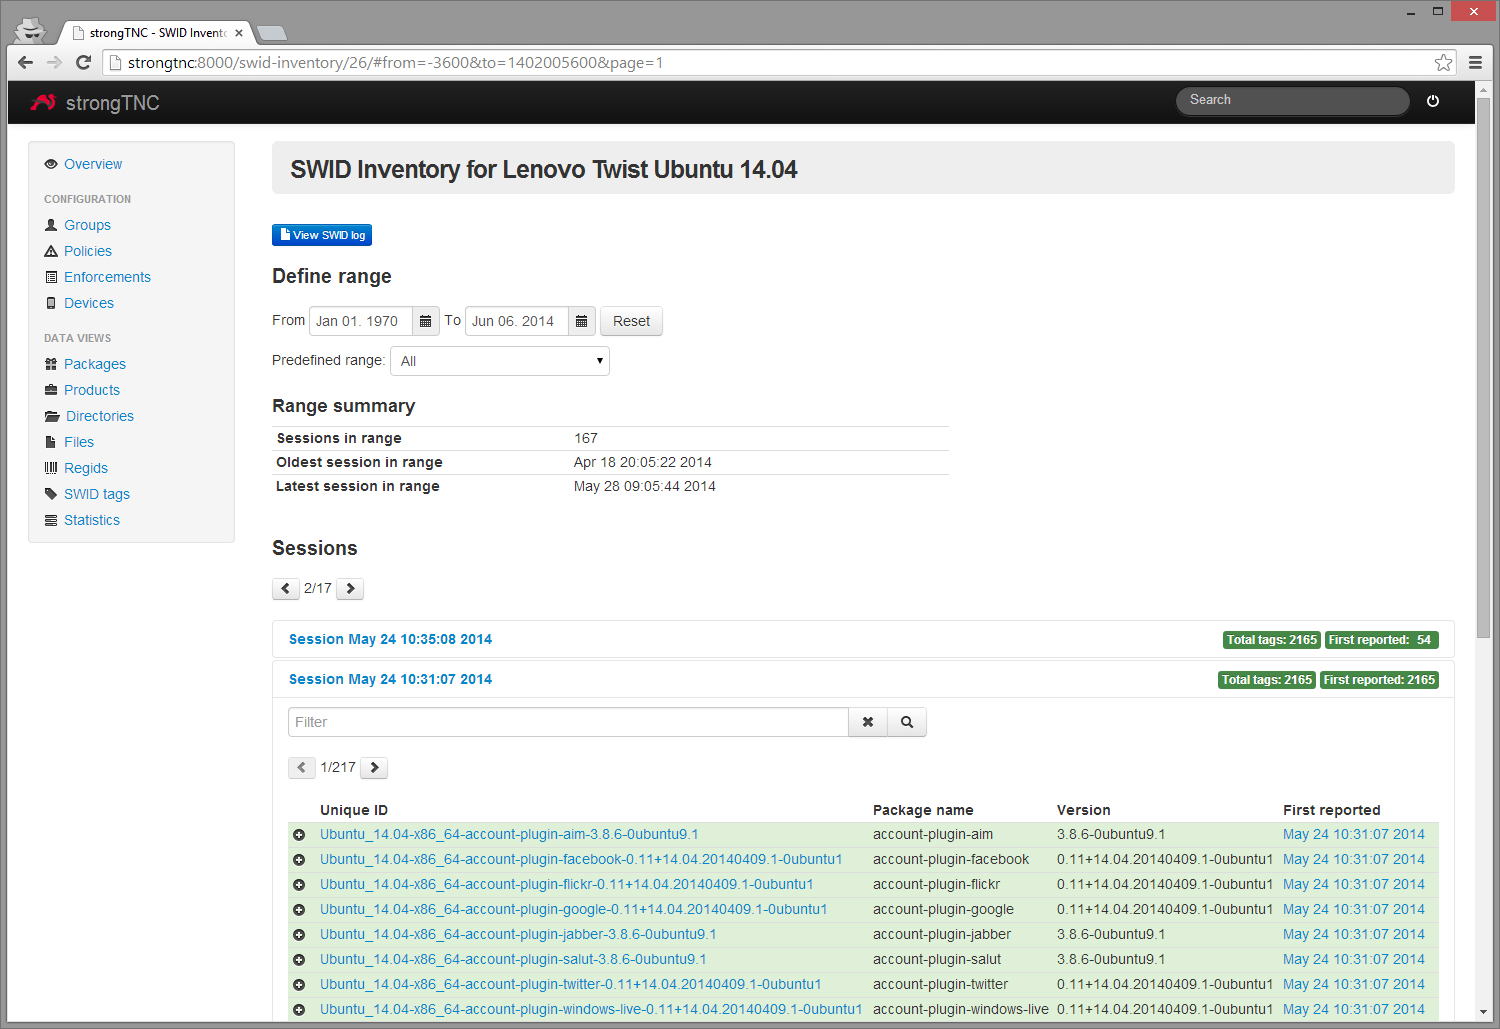
\includegraphics[width=0.8\textwidth]{./images/Views/inventory-view}
	\caption{SWID Inventory View}
	\label{fig:swid-inventory-view}
\end{figure}


\subsubsection{SWID Log View}
Die Log View zeigt den Verlauf der Installation und Entfernung von Software
Paketen auf einem ausgewählten Gerät (\nameref{strongTNC:UC01}).\\
Da bei jeder SWID Messung jeweils alle vorhanden SWID Tags übermittelt werden,
lässt sich für jedes Paket sagen, wann es installiert, beziehungsweise entfernt
wurde. Um diese Information zu erhalten muss der Tag Bestand von zwei zeitlich
aufeinander folgenden Sessions verglichen werden, die Differenz der Mengen zeigt
die Veränderung des Installationsverlaufes an.

\begin{figure}[H]
	\centering
	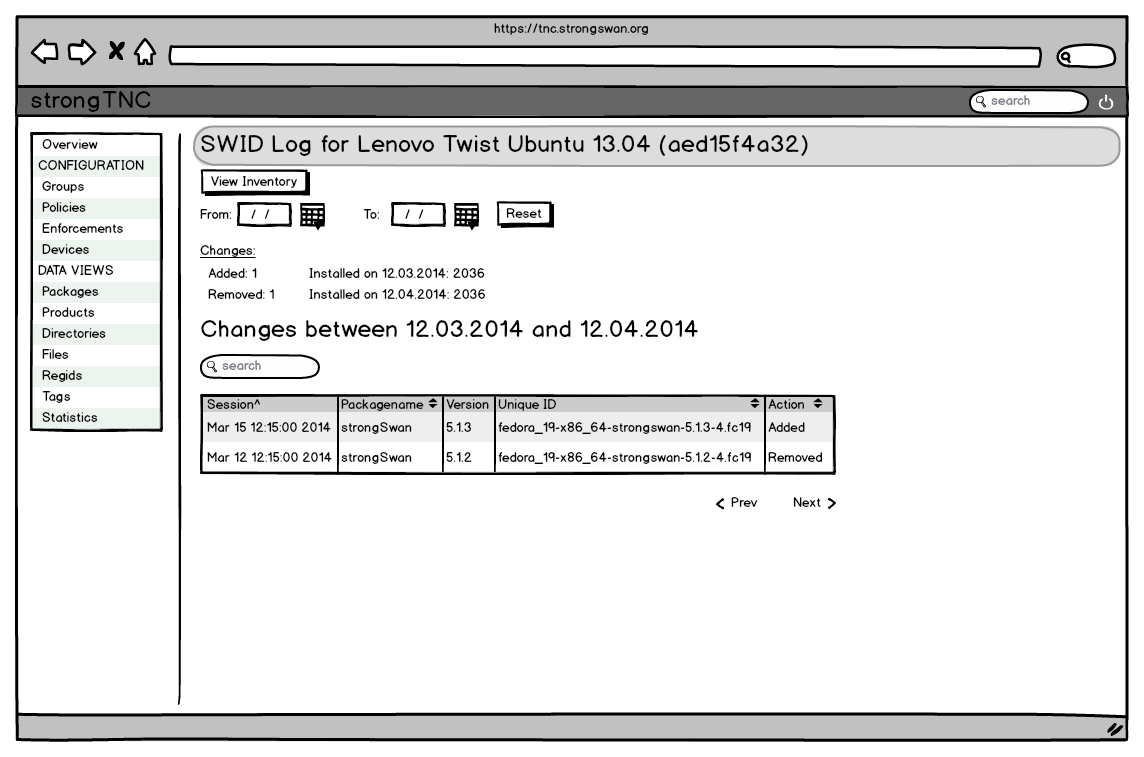
\includegraphics[width=0.8\textwidth]{./images/mockups/swid-log}
	\caption{SWID Log View Mockup}
	\label{fig:swid-log}
\end{figure}

\begin{figure}[H]
	\centering
	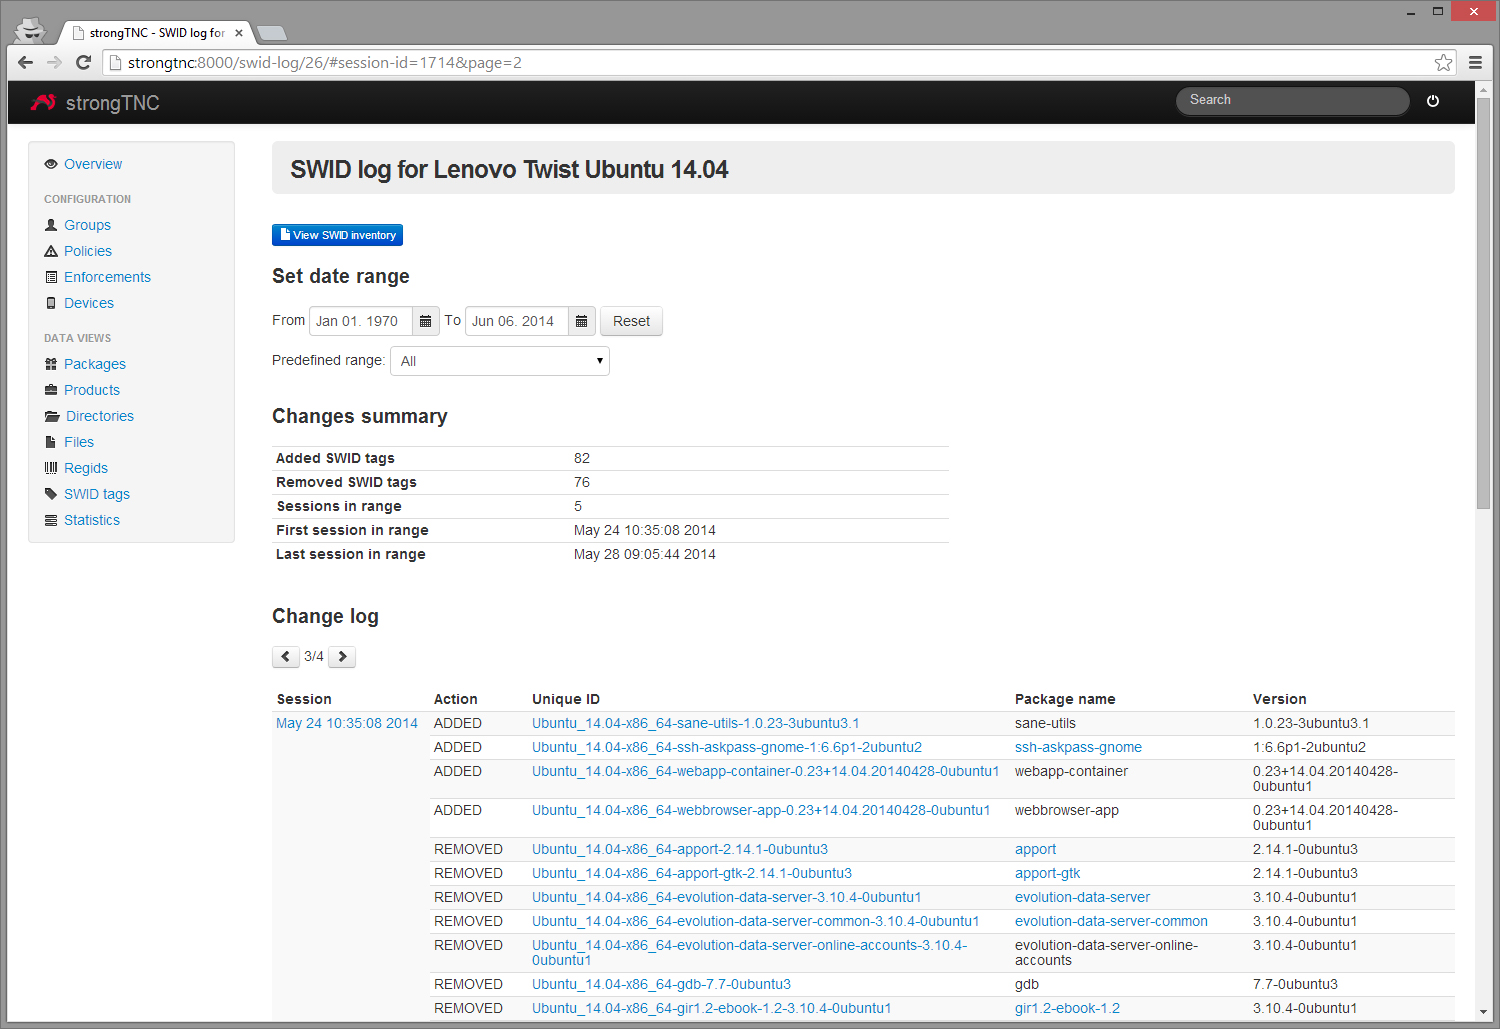
\includegraphics[width=0.8\textwidth]{./images/Views/log-view}
	\caption{SWID Log View mit Details für eine ausgewählte Session}
	\label{fig:log-view}
\end{figure}